\documentclass[12pt,a4paper]{article}
\usepackage[utf8]{inputenc}
\usepackage[czech, english]{babel}
\usepackage[T1]{fontenc}
\usepackage{amsmath}
\usepackage{amsfonts}
\usepackage{amssymb}
\usepackage{graphicx}
\usepackage[final,pdftex, colorlinks=false]{hyperref}
\usepackage{xcolor}
\usepackage{comment}
\usepackage{todonotes}
\usepackage{floatrow}
\usepackage{multirow}

\usepackage{listings}			%vkladani kodu
\lstset{basicstyle=\scriptsize,
  showstringspaces=false,
  commentstyle=\color{red},
  keywordstyle=\color{blue},
  breaklines=true
}

%okraje
\usepackage[
left=35mm,
right=25mm,
top=40mm,
bottom=35mm]
{geometry}

\author{Adam Laža}

%%%%%%%%%%Prikazy%%%%%%%%%%
\renewcommand\baselinestretch{1.3}		%radkovani
\parskip=0.8ex plus 0.4ex minus 0.1 ex	%mezera mezi odstavci

\newcommand{\keywords}[2]{\noindent\textbf{#1: }#2}

\newcommand{\necislovana}[1]{%
\phantomsection
\addcontentsline{toc}{section}{#1}

\newcommand{\exedout}{%
  \rule{0.8\textwidth}{0.5\textwidth}%
}


\section*{#1}
\markboth{\uppercase{#1}}{}
}
%%%%%%%%%%%%%%%%%%%%%%%%%%%%

%%%%%%%%%%Zahlavi%%%%%%%%%%%
\usepackage{fancyhdr}
\fancyhead[L]{ČVUT v~Praze}
\setlength{\headheight}{16pt}
%%%%%%%%%%%%%%%%%%%%%%%%%%%%

\begin{document}
\pagestyle{empty}

\newpage
\begin{center}
%napisy
\newcommand{\napisCVUT}{České vysoké učení technické v Praze}
\newcommand{\napisFS}{Fakulta stavební}
\newcommand{\napisObor}{Obor geodézie, kartografie a geoinformatika}
\newcommand{\napisKatedra}{Katedra geomatiky}
\newcommand{\napisVedouci}{Vedoucí práce: Ing. Martin Landa, Ph.D.}
\newcommand{\napisAutor}{Adam Laža}
\newcommand{\napisDatum}{Praha 2015}
\newcommand{\napisNazevI}{Interpolace metodou přirozeného souseda}
\newcommand{\napisNazevAjI}{Natural neighbour interpolation}
\newcommand{\napisBakalarka}{Bakalářská práce}
\newcommand{\napisPraha}{Praha 2015}
%
% prikazy
%\newcommand{\velka}[1]{\uppercase{#1}}
\newcommand{\velka}[1]{\textsc{#1}}
%
% 
\newif\ifpatitul
\patitultrue

\ifpatitul
{\Large\velka{\napisCVUT}}\\
\velka{\Large\napisFS}\\
\vfill
{\LARGE\velka{\napisBakalarka}}
\vfill
{\large\napisPraha\hfill\napisAutor}
\newpage
\fi%patitul


{\Large\velka{\napisCVUT}}\\
{\Large\velka{\napisFS}}\\
{\Large\velka{\napisObor}}
\vfill

\includegraphics[width=3cm]{logo_cvut_cb} %~
\vfill
{\Large\velka{\napisBakalarka}}\\
\Large\velka{\napisNazevI}\\
\large\velka{\napisNazevAjI}
\vfill
{\large%
\napisVedouci\\
\napisKatedra\\
\bigskip
\napisDatum\hfill\napisAutor}
\end{center}


\newpage
\begin{abstract}
\bigskip
Cílem této bakalářské práce je návrh a implementace nástroje pro interpolaci metodou přirozeného souseda pro GRASS GIS 7. Starší verze GRASS GIS 6 sice tuto metodu nabízí v rámci volitelně doinstalovatelných balíčků Add-Ons, ale jako modul napsaný v Bashi a s vnitřní závislostí na knihovně \textit{nn-c}. Tato knihovna obsahuje knihovnu \textit{Triangle}, která nedovoluje zařazení tohoto nástroje do oficiální distribuce GRASS GISu.

V rámci této bakalářské práce byl modul přepsán do jazyka Python, tak aby vyhovoval verzi 7. Práce se dále zabývá možnostmi budoucí implementace knihovny v jazyce C bez závislosti na knihovně \textit{Triangle}, tak aby mohl tento interpolační nástroj zařazen do oficiální distribude GRASS GISu.
Část textu této práce se dále zabývá porovnání rychlosti a kvality výstupu mezi GRASS GISem a ostatními gisovými softwary.

\bigskip
\keywords{Klíčová slova}{GIS, GRASS GIS, interpolace, přirozený soused, Delaunayho triangulace, Voronoiovy polygony}

\end{abstract}

\selectlanguage{english}
\begin{abstract}
\bigskip
The aim of this bachelor thesis is the project and the implementation of a tool for a natural neighbour interpolation pro GRASS GIS 7. Previous version GRASS GIS 6 contains such a tool as a optional package of Add-Ons, but this modul is written in Bash and with inner dependency on \textit{nn-c} library. Due to this library contains \textit{Triangle} library which is not under the GNU GPL licence it is not possible to add the interpolation tool into official GRASS GIS distribution.

\bigskip
\keywords{Keywords}{GIS, GRASS GIS, natural neighbour interpolation, Delaunay triangulation, Voronoi's polygons}

\end{abstract}
\selectlanguage{czech}

\newpage
\tableofcontents

\newpage
\pagestyle{fancy}

\necislovana{Úvod}
V reálném životě se většinou nesetkáváme s případem, kdy pro naši oblast zájmu, ať už se jedná o interval, plochu nebo prostor, máme dostatek bodových dat o daném jevu. Mnohem častěji máme k dispozici pouze soubor bodových dat, která jsou buď náhodně nebo uspořádaně rozmístěna po naší oblasti zájmu. Fyzické zhuštění takovéto sítě a sběr dalších dat může být časově či finančně náročné, příliš obtížné nebo v rámci možností metod zcela nereálné.

Obvykle ovšem potřebujeme znát hodnotu daného jevu i mimo měřené body, nejčastěji pro celé zájmové území. V takovéto chvíli se musíme použít nějaký interpolační nástroj, který vypočte přibližnou hodnotu v území mezi měřenými body. Jako příklad může být uvedeno vytvoření výškopisu, či DMT pro území, kde máme k dispozici data o výšce v pravidelné mřížce nebo teplotní mapa na základě údajů z nepravidelně rozmístěných meteostanic.

V této práci se budu zabývat interpolací přirozeného souseda a její implementací do GRASS GISu 7\footnote{\url{http://grass.osgeo.org}}. 


\newpage
\section{GRASS GIS}
GRASS (Geographic Resources Analysis Support System) GIS je geografický informační systém pro správu a analýzu prostorových dat, obrazových záznamů, produkci map a grafických výstupů, prostorové modelování a 3D vizualizaci. Na mnoha platformách (GNU/Linux, MS Windows, MAC OS) umožňuje práci s rastrovými i vektorovými daty a to buď pomocí příkazové řádky nebo grafického uživatelského rozhraní. GRASS GIS je otevřený a volně šiřitelný software pod licencí GNU GPL.

Historie\footnote{Praktická rukověť ke geografickému informačnímu systému GRASS \url{http://geo.fsv.cvut.cz/data/grasswikicz/grass_prirucka/grass_prirucka_0.4.pdf}} GRASS GISu začíná v roce 1982, kdy začal být vyvíjen U.S. Army Corps of Enginneer/CERL (Construction Engineering Research Lab) pro vojenské účely. Nicméně koncem osmdesátých let byly veškeré zdrojové kódy dány k dispozici veřejnosti. Na začátku devadesátých let se začal pomocí internetu celosvětově rozšiřovat. V roce 1995 CERL odstoupil od projektu a vývoje se ujal GRASS Development Team, který zahrnoval odborníky z celého světa.

GRASS je jeden z nejznámějších open-source GIS softwarů, jehož vývoj trvá déle než třicet let. Jádro softwaru je napsáno v jazyce C. Avšak snahou vývojářů je rozšíření GRASSu mezi širší odbornou veřejnost a proto v rámci snadnějšího použití jsou do programu začleněny moduly napsané v jazyce Python nebo C. Aktuálně je k dispozici verze 7, na jejímž vývoji se podílí několik vývojářů z řad dobrovolníků po celém světe.

\subsection{GRASS GIS Add-Ons}
GRASS GIS je od roku 1982 v neustálem vývoji. Síla a úspěch GRASS GISu je založená hlavně na komunitě uživatelů. S ohledem na to, je filozofií vývojového týmu GRASS GISu vést uživatele k tvorbě jejich vlastních nástrojů a aplikaci pro GRASS GIS. Pokud uživatel vyvine nějaký nástroj, který by mohl být užitečný ostatním uživatelům má možnost svůj kód zveřejnit a zpřístupnit ostatním uživatelům.

\newpage
\section{Delaunayova triangulace}
Interpolace metodou přirozeného souseda vychází z Delanayovi triangulace(DT) či Voronoiových diagramů(VD). Jak DT či VD jsou důležité konstrukce ve výpočetní geometrii. Delaunayova triangulace lze odvodit z Voronoiových diagramů a stejně tak Voronoivy diagramy se dají naopak odvodit z Dalunayovi triangulace.

\subsection{Triangulace obecně}
\todo[inline]{Vkladat definici?}
\textbf{Definice:}
Triangulace $\Delta$ nad množinou bodu $P$ představuje takové planární rozdělení, které vytvoří soubor $m$ trojúhelníků $t = \{ t_1, t_2,...,t_m \}$ a hran tak, aby platilo:

Libovolné dva trojúhelníky $t_i$,$t_j \in \Delta, (i \neq j)$, mají společnou nejvýše hranu.

Sjednocení všech trojúhelníků $t \in \Delta$ tvoří doménu $\Omega$.

Uvnitř žádného trojúhelníku neleží žádný další bod z P.

\bigskip
Triangulace má širokou škálu aklikací. V kartografii a GISech se využívá pro tvorbu DMT. V DPZ lze využít pro tvorbu prostorových modelů, své uplatnění najde také v počítačové grafice a vizualizaci prostorových dat a mnoho dalších.

V našem případě budeme triangulaci provádět uvnitř takzvaného \textit{konvexního obalu}. Konvexní obal množiny bodů $P$ představuje takový konvexní mnohoúhelník, který obsahuje všechny body množiny bodů P, má co nejmenší plochu a ve kterém zároveň spojnice mezi kterýmikoliv body množiny bodů $P$ leží uvnitř obalu.
\todo[inline]{obrazek konvex hullu, domeny}

\begin{figure}[h!]
\centering
\begin{floatrow}
\ffigbox{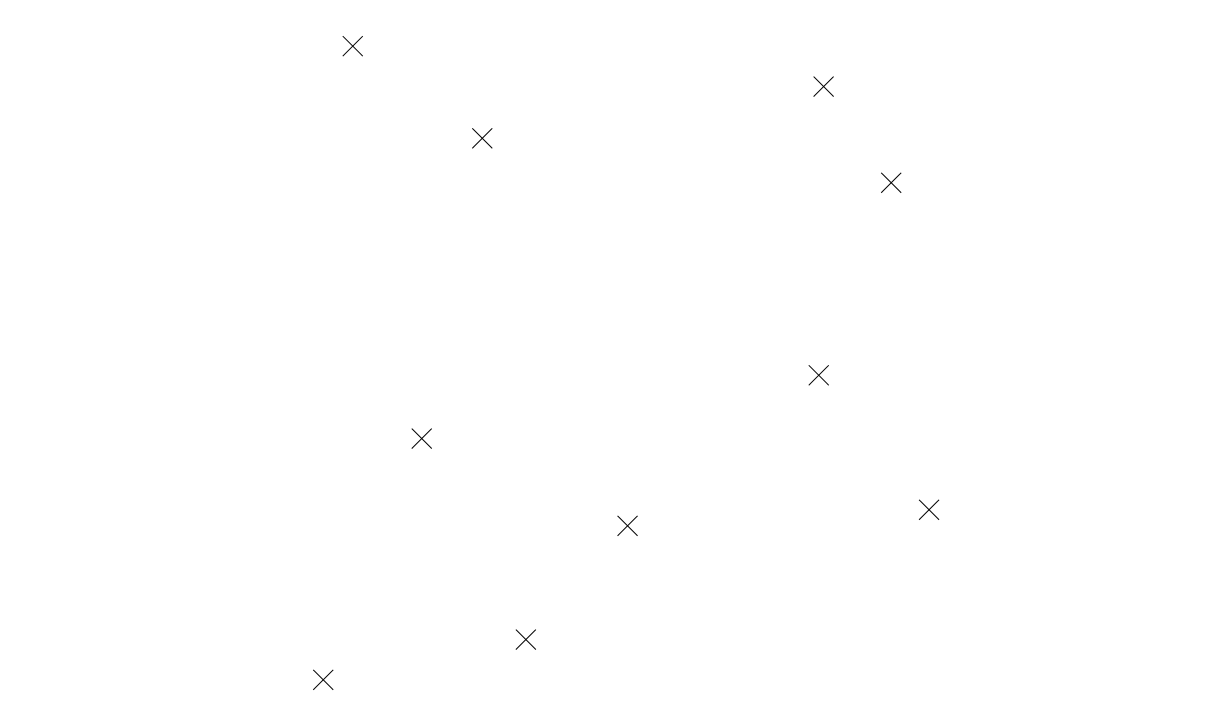
\includegraphics[width=0.48\textwidth]{../img/body.png}}{\caption{Soubor bodů}}{\label{fig:soubor_bodu}}
\ffigbox{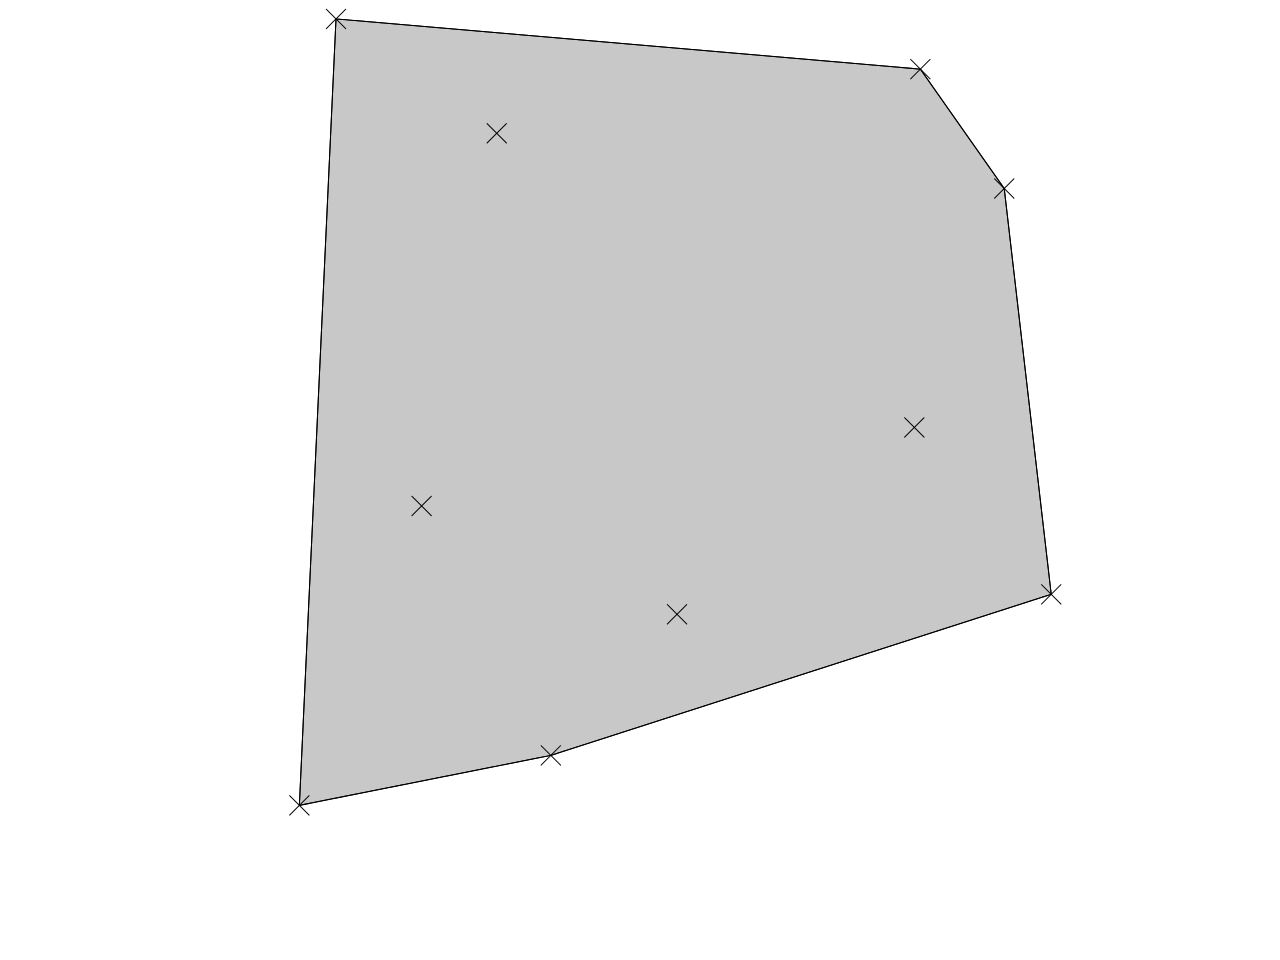
\includegraphics[width=0.48\textwidth]{../img/domain.png}}{\caption{Konvexní obal nad doménou $\Omega$ }}{\label{fig:domena}}
\end{floatrow}
\end{figure}

\newpage
\subsection{Validní a regulérní triangulace}
V podstatě by se dalo říct, že triangulace je jakákoliv trojúhelníkoví síť mezi body v prostoru. Tato práce se však bude zabývat triangulační sítí se specifickými vlastnostmi.

\todo[inline]{pridat obrazky pro jednotlive podminky}
\begin{enumerate}
\item Žádný z trojúhelníků $t_{ijk}$ není zdegenerovaný, tzn. že vrcholy \textit{i,j,k} neleží na přímce.
\item Žádná dvojice trojúhelníků se nepřekrývá, tzn $Int(t_{ijk}) \cap Int(t_{lmn}) = \emptyset$
\item Hranice dvou trojúhelníků se setkávají pouze na jejich hranách nebo v jejich vrcholech.
\item Sjednocení všech trojúhelníků v celé triangulační síti se rovná celé doméně $\Omega$, nad kterou triangulaci provádíme.
\item Doména $\Omega$ musí být spojitá.
\item Triangulační síť nesmí obsahovat díry.
\item Jestliže vrchol $v_i$ leží na hranici konvexního obalu, pak musí existovat právě dvě hraniční hrany, které mají vrchol $v_i$ jako společný vrchol. To mimo jiné znamená, že počet hraničních vrcholů je roven počtu hraničních hran.
\end{enumerate}

Pokud jsou naplněny první čtyři podmínky, může se triangulace nazvat \textit{validní}. V případě, že naplníme všech sedm podmínek, dá se mluvit o \textit{regulérní} triangulaci.
\todo[inline]{obrazek validni/regulerni triangulaci}

\newpage
\begin{figure}[h!]
\centering
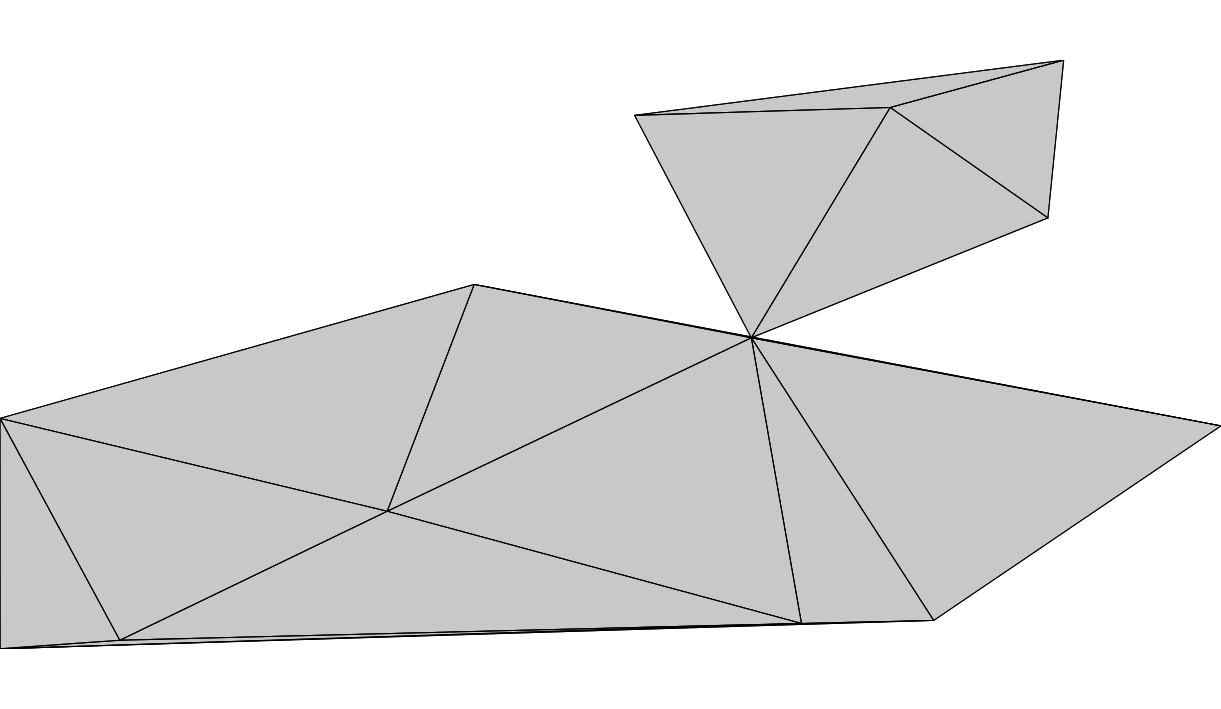
\includegraphics[width=0.9\textwidth]{../img/vnr.png}
\caption{Triangulace validní, ale neregulérní}
\label{fig:trian_valid_not_reg}
\end{figure}

V případě triangulace na Obrázku \ref{fig:trian_valid_not_reg} se jedná o triangulaci validní, neboť splňuje všechny z prvních čtyř podmínek. Nicméně nesplňuje podmínku č. 7, neboť existují více jak právě dvě hraniční hrany, které vstupují do jednoho vrcholu na konvexním obalu, a triangulaci tedy nelze nazvat i regulérní.

\begin{figure}[h!]
\centering
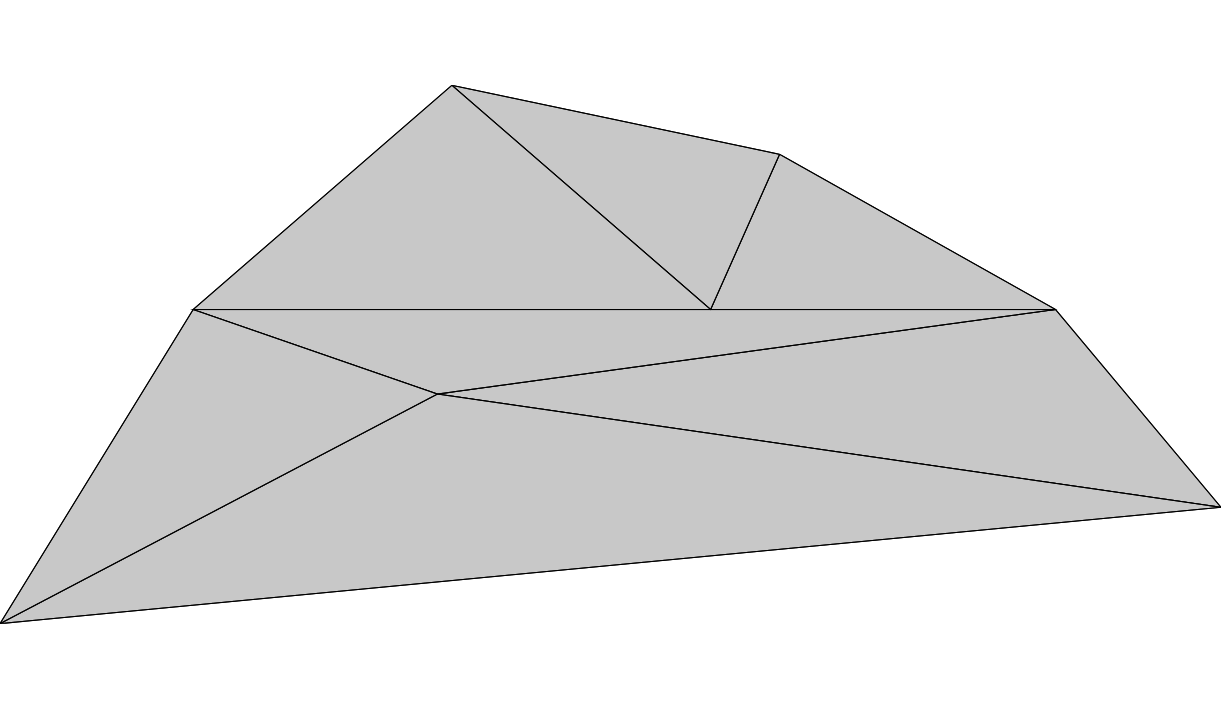
\includegraphics[width=0.9\textwidth]{../img/nv.png}
\caption{Triangulace nevalidní}
\label{fig:train_not_valid}
\end{figure}

Triangulace na Obrázku \ref{fig:train_not_valid} není validní, protože nesplňuje podmínku č. 3. Tím pádem se nejedná ani o triangulaci regulérní.

\newpage
\begin{figure}[h!]
\centering
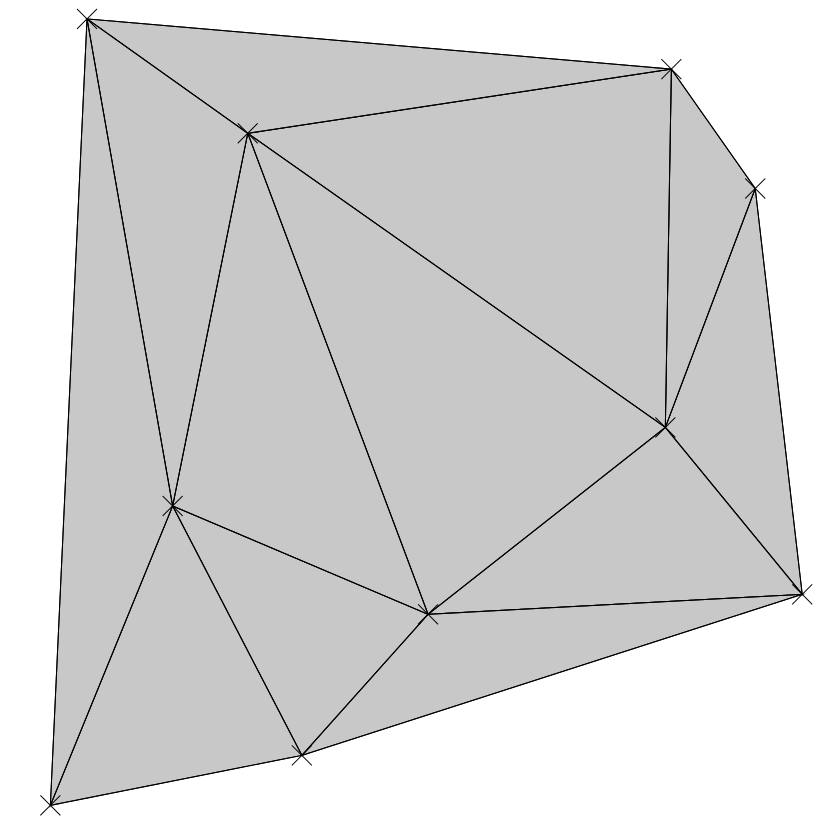
\includegraphics[width=0.9\textwidth]{../img/triangulation.png}
\caption{Regulérní triangulace}
\label{fig:triangulace}
\end{figure}

Na Obrázku \ref{fig:triangulace} už můžeme vidět validní a regulérní triangulaci. Jedná se též o triangulaci \textit{optimální}, což je termín, kterým se budeme zabývat v další kapitole.

\newpage
\subsection{Optimální triangulace}

Nad doménou $\Omega$ neexistuje pouze jediná trojúhelníková síť, v závislosti na počtu bodů v množině a jejich konfiguraci existuje poměrně velké množství možností, jak může trojúhelníková síť vypadat. Ne všechny sítě jsou však vhodné k dalšímu zpracovávání, a právě proto je snaha najít \textit{optimální} triangulaci.

Při řešení otázky, jak vypadá optimální triangulace, je zásadní zamyslet se nad tvarem trojúhelníků. V ideálním případě by byly všechny trojúhelníky rovnostranné, leč tento případ se v případě náhodně roztroušených dat nevyskytuje.

Při tvorbě optimální triangulace se tedy problém řeší z opačného konce. Zásadní snahou při tvorbě sítě by mělo být vyhýbání se podlouhlým, štíhlým nebo téměř degenerovaným trojúhelníkům, tedy trojúhelníkům s příliš ostrými nebo s příliš tupými úhly. 

\paragraph{Kruhová podmínka}
Definice:
Nechť hrana $\overline{p_ip_j}$ inciduje s trojúhelníkem $t_1$ tvořeným vrcholy $p_i,p_j,p_k$ a trojúhelníkem $t_2$ tvořeným vrcholy $p_i,p_j,p_l$ a kružnice $k$ procházející body $p_i,p_j,p_k$. Hrana $\overline{p_ip_j}$ je nelegální tehdy a právě jen tehdy, jestliže bod $p_l$ leží uvnitř $k$.

Pokud tedy bod $p_l$ leží uvnitř kružnice $k$, je hrana $\overline{p_ip_j}$ a tedy diagonála čtyřúhelníku nelegální, stejně tak jako oba trojúhelníky $t_1$ a $t_2$. K jejich legalizaci je provést tzv. \textit{Edge swaping}.

\paragraph{MaxMin a MinMax úhlová podmínka}

Pokud nad množinou bodů P provedeme všechny možné triangulace, můžeme nejoptimálnější triangulaci určit pomocí MaxMin popř. MinMax podmínky. V případě MaxMin podmínky je pro každou možnou triangulaci nalezen největší minimální vnitřní úhel trojúhelníku a ten je porovnán s největším minimálním úhel ostatních triangulací, což vede k eliminaci trojúhelníků s velmi tupými úhly. U MinMax podmínky se postupuje obdobně, pouze se porovnávají nejmenší maximální vnitřní úhly trojúhelníků a eliminují se tak trojúhelníky s velmi ostrými úhly.

\todo[inline]{Vložit definici?}
\todo[inline]{úhel alfa a triangulace s čarou}
MinMax podmínka:
Eliminace trojúhelníků s příliš tupými úhly. Triangulace $\Delta(P)$ je vzhledem k tomuto kritériu na rozdíl od triangulace $\Delta^{'}(P)$ optimální, je–li největší úhel $\alpha$ generovaný triangulací $\Delta(P)$ menší než největší úhel $\alpha^{'}$ generovaný triangulací $\Delta^{'}(P)$.

$\alpha_{max} = max(\alpha_i(\Delta))$

$\alpha^{'}_{max} = max(\alpha_i^{'}(\Delta))$

$\alpha_{max} < \alpha^{'}_{max}$

\bigskip
MaxMin podmínka:
Eliminace trojúhelníků s příliš ostrými úhly. Triangulace $\Delta(P)$ je vzhledem k tomuto kritériu na rozdíl od triangulace $\Delta^{'}(P)$ optimální, je–li nejmenší úhel $\alpha$ generovaný triangulací $\Delta(P)$ větší než nejmenší úhel $\alpha^{'}$ generovaný triangulací $\Delta^{'}(P)$.

$\alpha_{min} = min(\alpha_i(\Delta))$

$\alpha^{'}_{min} = min(\alpha_i^{'}(\Delta))$

$\alpha_{min} > \alpha^{'}_{min}$

\paragraph{Neutrální případ pro MaxMin podmínku}

Problém nastává ve chvíli, kdy některé body, mezi kterými chceme triangulaci provést, leží na kružnici nebo se tomu limitně blíží. v takových chvílí nastává takzvaný neutrální případ pro MaxMin podmínku. V některých případech to může vést k nejednoznačnému určení, která z triangulací je optimální a musíme si pomoci hodnocením na základě nejen MaxMin ale i MinMax podmínky.

\begin{figure}[h!]
\centering
\begin{floatrow}
\ffigbox{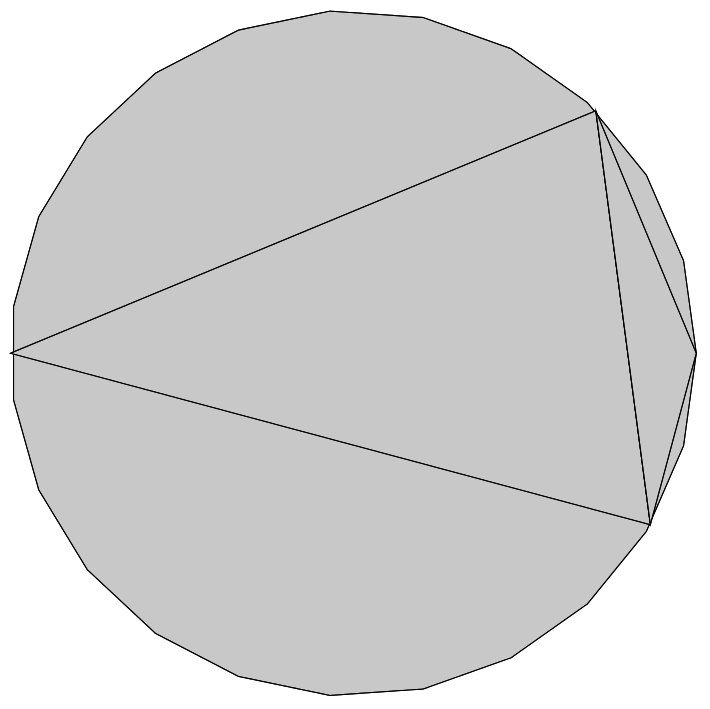
\includegraphics[width=0.48\textwidth]{../img/minmax2.png}}{\caption{Případ1}}{\label{fig:neutral_case_1}}
\ffigbox{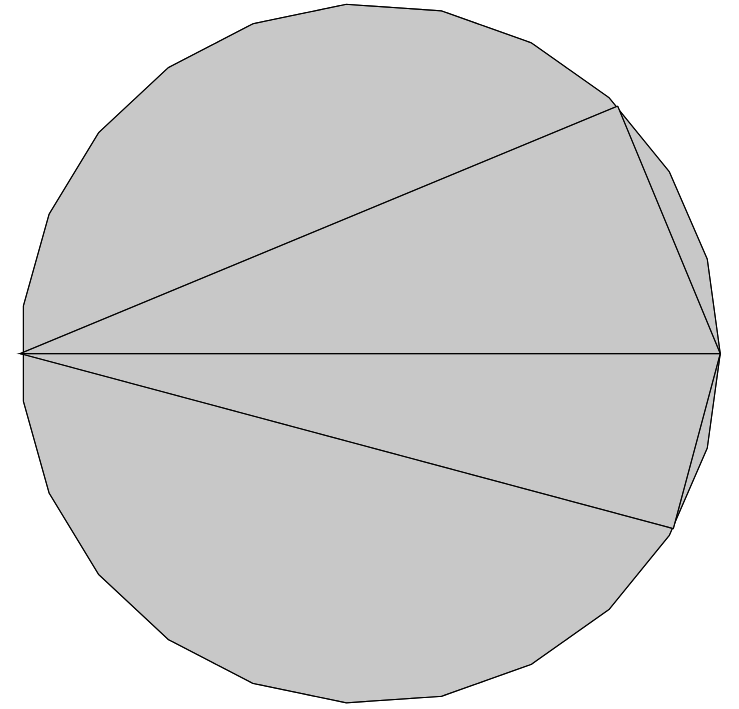
\includegraphics[width=0.48\textwidth]{../img/minmax1.png}}{\caption{Případ2}}{\label{fig:neutral_case_2}}
\end{floatrow}
\end{figure}
\todo[inline]{Obrázky z GRASSu, jak udělat skutečnou kružnici, označení úhlů}
Nejčastěji tento jev nastává u čtyřúhelníků, jejichž všechny vrcholy leží na kružnici. Jak můžeme vidět na Obrázcích \ref{fig:neutral_case_1} a \ref{fig:neutral_case_2} v obou případech je maximální minimální úhel triangulace obvodový úhel nejkratší strany čtyřúhelníku. V tomto případě se tedy jedná o neutrální případ pro MaxMin podmínku. Pokud bychom tedy triangulaci vyhodnocovali pouze na základě MaxMin podmínky mohly bychom obě triangulace prohlásit za optimální. Už od pohledu je ale zřejmé, že lepší tvar trojúhelníků poskytujeme triangulace nalevo. Pokud ale triangulace hodnotíme i s ohledem na MinMax podmínknu, můžeme prokázat, že triangulace na Obrázku \ref{fig:neutral_case_2} je optimální.

\paragraph{Edge swaping, legalizace}
Na Obrázcích \ref{fig:neutral_case_1} a \ref{fig:neutral_case_2} jsme si ukázali případ neutrálního případu pro MinMax podmínku. Proces, při kterém jsme zaměnili diagonálu čtyřúhelníku tak, aby byli oba trojúhelníky lokálně optimální, se nazýva \textit{Edge swaping.} Pokud budeme tento proces aplikovat pro celou triangulaci dojde k takzvané \textit{legalizaci} triangulace.

\newpage
\section{Voronoiovy diagramy}

Voronoiovy diagramy úzce souvisí s Delaunayovou triangulací. Představme si opět množinu bodů $P = \{p_1,...p_N\} $ v rovině $E^2$ a nechť je $d(p_i,p_j) $ Eukleidovská vzdálenost mezi body $p_i$ a $p_j$. Rovinu po té rozdělíme na oblasti $V(p_i,...,p_N)$, kde každému bodu $p_i$ z množiny $P$ přiřadíme takovou oblast, která splňuje následující podmínku: 

$V(p_i) = \{ x: d(x, p_i) < d(x, p_j), j = 1,...,N\}$.

Pro každou takovouto oblast přiřazenou bodu $p_i$ po té platí, že všechny body uvnitř této oblasti jsou k bodu $p_i$ blíž než ke kterémukoliv jinému bodu z množiny $P$. Toto rozdělení roviny se nazývá \textit{Voronoiův diagram (VD)} množiny bodů a každá uzavřená buňka se nazývá \textit{Voronoiova buňka.}

\bigskip
Voronoiův diagram má následující vlastnosti: 
\begin{enumerate}
\item Voronoiův diagram pro množinu bodů je pouze jeden.
\item Všechny oblasti jsou konvexní.
\item Oblast $V(p_i)$ obsahuje jediný bod $p_i \in P$.
\item Oblasti na okraji jsou neohraničené.
\item Počet hran a uzlů je přímo úměrný počtu bodů v množině P.
\item Pokud žádné 4 body neleží na kružnici, uzly mají stupeň 3.
\item Uzel leží ve středu kružnice určené 3 body z P, které leží v přilehlých oblastech a neleží na přímce.
\end{enumerate}

\begin{figure}[h!]
\centering
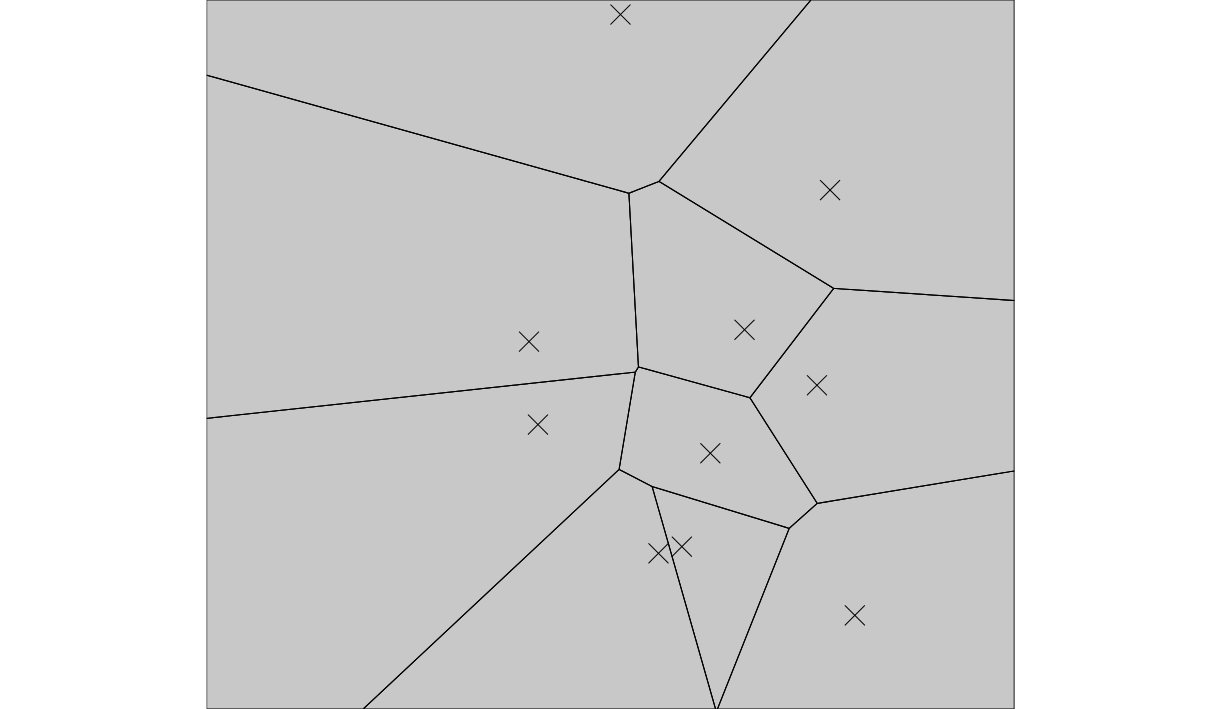
\includegraphics[width=0.9\textwidth]{../img/vor_pol.png}
\caption{Voronoivy polygony}
\label{fig:vor_pol}
\end{figure}

Nechť $H(p_i,P_j)$ je polorovina obsahující všechny body v rovině, jejichž vzdálenost od bodu $p_i$ je menší než od bodu $p_j$. Potom Voronoiova oblast $V(p_i)$ je průnikem N-1 polorovin,
$V(p_i)= \bigcap\limits_{\substack{j=1,...,N \\ i\not=j}}H(p_i,p_j)$, kde každá oblast má maximálně N-1 stran.

Z Obrázku \ref{fig:vor_pol} je vidět, že oblasti přiřazené pro body na okraji konvexního obalu nejsou zcela ohraničené a uzavřené. Jednotlivé hranice oblastí nazýváme \textit{Voronoiovi polygony}, které jsou složeny z takzvaných \textit{Voronoiových hran a bodů}. O dvou bodech $p_j$ a $p_k$ můžeme tvrdit, že jsou \textit{Voronoiovi sousedé}, pokud oblasti, kterým náleží, sdílí společnou \textit{Voronoiovu hranu}. 

Občas se můžeme setkat i s označením \textit{Thiessenovy polygony} podle klimatologa Thiessena, který Voronoiovi diagramy používal k interpolaci klimatických dat z náhodně distribuovaných meteorologických stanic.

\newpage
\subsection{Voronoiovy diagramy a Delaunayova triangulace}

DT je planární graf, který je duální k VD. Jedna konstrukce tedy může být odvozena od druhé a naopak. 
Pokud pro množinu bodů v rovině provedeme rozdělení do Voronoiových diagramů a následně spojíme úsečkami všechny Voronoiovi sousedy získáme Delaunayovu triangulaci.

\begin{figure}[h!]
\centering
\begin{floatrow}
\ffigbox{
\includegraphics[width=0.45\textwidth]{../img/vd_vor.png}}{\caption{Voronoiův diagram souboru bodů}}{\label{fig:vd_vor}}
\ffigbox{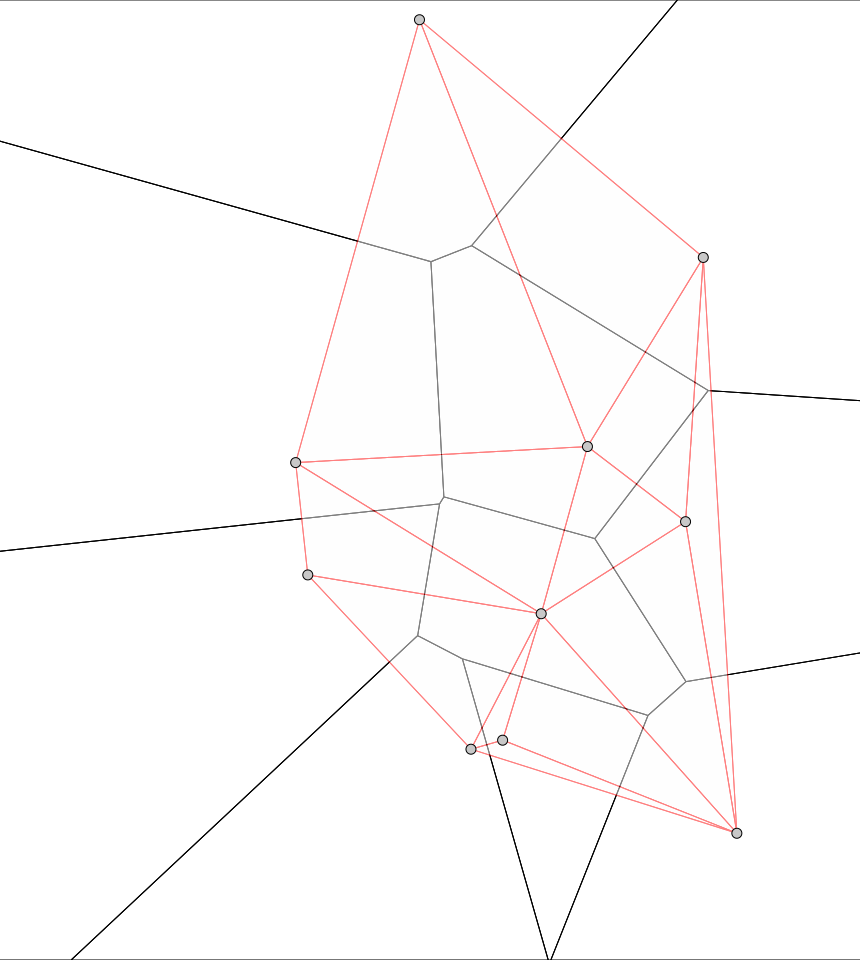
\includegraphics[width=0.45\textwidth]{../img/vd_del.png}}{\caption{Voronoiův diagram a Delaunayova trinagulace}}{\label{fig:vd_del}}
\end{floatrow}
\end{figure}

Na Obrázku \ref{fig:vd_vor} můžeme vidět Voronoiův diagram pro množinu bodů. Pokud každou dvojici Voronoiových sousedů spojíme spojnicí, jak je vidět na Obrázku \ref{fig:vd_del} získáme několik trojúhelníků, které se nepřekrývají a tvoří trojúhelníkovou síť. Spojnice mezi body, které jsou přiřazeny k neuzavřeným oblastím, tvoří konvexní obal. Pro trojúhelníkovou síť uvnitř tohoto konvexního obalu se jedná o Delaunayovu triangulaci.

Trojúhelníky této sítě se nazývají \textit{Delaunayovi trojúhelníky}, které jsou tvořeny spojnicemi tzv. \textit{Delaunayvými hranami}. Dále je také zřejmé, že Voronoiovy hrany leží na ose Delaunayových hran.


\newpage
\section{Algoritmy pro tvorbu DT}
\todo[inline]{Obrázky pro algoritmy}
Triangulační algoritmy jsou poměrně dobře matematicky prozkoumaná oblast, ke které máme k dispozici široký teoretický základ. Při hledání vhodného algoritmu musíme zohlednit následující požadavky:
\begin{itemize}
\item Jednoduchost algoritmu a jeho snadná implementace.
\item Dostatečná rychlost i pro velké množiny bodů (n>1E6), ideálně aby se výpočetní čas blížil $O(n . log(n))$.
\item Malá citlivost a vysoká stabilita pro případy nejednoznačné triangulace (body na kružnici).
\item Převod do vyšších dimenzí.
\item Možnost paralelizace algoritmu.
\end{itemize}
Vhodný algoritmus je třeba vybírat na základe datových struktur a konkrétním případu. Ne vždy lze dokonale splnit všechny požadavky, např. jednoduché implementace mají delší výpočetní čas. Naopak algoritmy s kratším výpočetním časem jsou dost náročné na implementaci.

\subsection{Lokální optimalizace}
\textit{Lokální optimalizace (LO)} je proces přetvoření libovolné triangulace DT. Proces je prováděn pomocí prohazování nelegálních hran v dvojicích trojúhelníků tvořících konvexní čtyřúhelník na základě Kruhové nebo MaxMin podmínky.

Pro množinu bodu $P$ nechť $e_i$ je vnitřní hrana triangulace a $Q$ je čtyřúhelník tvořený dvěma trojúhelníky se společnou hranou $e_i$. Pomineme možnost, že čtyřúhelník je nekonvexní nebo že všechny body leží na kružnici. Po té za použití MaxMin nebo Kruhové podmínky rozhodněme, zda je třeba prohodit hranu $e_i$. V případě, že po použití Lokální optimalizace není potřeba prohodit hranu, můžeme ji prohlásit za lokálně optimální. V případě, že  budeme lokální optimalizaci používat opakovaně pro všechny hrany v triangulaci, dokud nebudou všechny hrany lokálně optimální, získáme optimální triangulaci.

\todo[inline]{Jak psát pseudokód??}
\begin{comment}
1. proveď náhodnou regulérní triangulaci $\Delta$ množiny bodů $P$
2. if je $\Delta$ lokálně optimální
	stop
3. zvol vnitřní hranu $e_i$ trinagulace $\Delta$
4. pokud je $e_i$ lokálně optimální
	goto 3.
5. prohoď $e_i$ za $e_i^1$ (přetvoř triangulaci $\Delta$ v triangulaci $\Delta^1$)
6. přiřaď $\Delta$:=$\Delta$
7. goto 2
\end{comment}


1. Vytvoř pomocnou triangulaci $\Delta(P)$.

2. legal=false

3. while $\Delta(P)$ !legal

4.\indent legal=true;

5.\indent Opakuj pro $\forall e_i \in \Delta(P)$

6.\indent \indent Vezmi hranu $e_i \in \Delta(P)$

7.\indent \indent Nalezni trojúhelníky $t_1,t_2$ incidující s $e_i$.

8.\indent \indent if $(t_1 \cup t_2)$ konvexní a nelegální

9.\indent \indent \indent  Legalize $(t_1,t_2)$

10.\indent \indent \indent legal=false;


\subsection{Paprskovitý algoritmus}

Tento algoritmus je podobný tomu předchozímu, pouze využívá jiný postup, jak nalézt počáteční triangulaci $\Delta$. Na začátku se nalezne bod $p$ z množiny $P$, takový který je nejbližší jejímu středu. Po té jej paprskovitě spojíme se všemi zbývajícími body množiny $P$. Tyto body se následně seřadí podle orientace a vzdálenosti od bodu $p$ a v tomto pořadí se spojí hranami. Potom se vytvoří hrany na hranici triangulace. Vzniklá triangulace se dále postupně po jednotlivých hranách legalizuje stejně jako v předchozím případě.


\subsection{Algoritmus inkrementálního vkládání}

Tento algoritmus je poměrně jednoduchý a snadný na implementaci, obzvlášť pokud je zvolena vhodná datová struktura. Jeho složitost je $0.(n^2)$, kterou lze úpravami zlepšit až na $0.(n.log(n))$. Tato metoda je tvořena třemi kroky. Na začátku je vytvořen konvexní obal množiny bodů $P$ a pro jeho lomové body se provede triangulace. Do vzniklé triangulace se postupně vkládají body z množiny $P$. Tato nově vzniklá triangulace nemusí být nutně DT a proto se provede ještě její legalizace.

\bigskip
1.  Vytvoření konvexního obalu $\Omega$ nad množinou bodů $P$.

2.  Vytvoř DT pro lomové body konvexního obalu.

3.  Opakuj pro $i \in 1,...,n$

4.\indent  Přidej p do DT.

5.\indent  Najdi trojúhelník $t$ s vrcholy $p_i, p_j, p_k$ takový, že $p \in t$

6.\indent  Jestliže $p$ leží uvnitř $t$:

7.\indent \indent Přidání hrany $\overline{p,p_i}$.

8.\indent \indent Přidání hrany $\overline{p,p_j}$.

9.\indent \indent Přidání hrany $\overline{p,p_k}$.

10.\indent \indent Legalizace hrany $p,\overline{p_i,p_j},t$.

11.\indent \indent Legalizace hrany $p,\overline{p_j,p_k},t$.

12.\indent \indent Legalizace hrany $p,\overline{p_k,p_l},t$.

13.\indent Jinak jestliže $p$ leží na hraně $p_i, p_j$ trojúhelníků $t_1, t_2$:

14.\indent \indent Přidání hrany $\overline{p,p_i}$.

15.\indent \indent Přidání hrany $\overline{p,p_j}$.

16.\indent \indent Přidání hrany $\overline{p,p_k}$.

17.\indent \indent Přidání hrany $\overline{p,p_l}$.

18.\indent \indent Legalizace hrany $p,\overline{p_j,p_k},t$.

19.\indent \indent Legalizace hrany $p,\overline{p_k,p_i},t$.

20.\indent \indent Legalizace hrany $p,\overline{p_i,p_l},t$.

21.\indent \indent Legalizace hrany $p,\overline{p_l,p_j},t$.


\subsection{Algoritmus inkrementální konstrukce (Step-by-Step)}

Tento postup je založen na postupném přidávání bodů do již vytvořené DT, tvoří triangulaci postupně, trojúhelník po trojúhelníku. Na začátku jsou vybrány dva body$p_1, p_2$, které jsou sami sobě Voronoiovými sousedy a mezi nimi je vytvořena základní Delaunayova hrana $e$. K této hraně $e$ se hledá další bod 	$p$, tak aby vyhovoval kruhové podmínce a který společně s hranou $e$ vytvoří Delaunayův trojúhelník s vrcholy $p_1, p_2$ a $p$, který se zapíše do DT. Každá Delaunayovská hrana je orientována, bod $p$ hledáme pouze vlevo od ní.Pro konstrukci se používá modifikovaná datová struktura AEL (Active Edge List).Obsahuje hrany $e$, ke kterým hledáme body $p$, do struktury se neukládá topologický model (viz kapitola \ref{sec:data_struct}).

Základní vlastnost toho postupu je, že se v každém kroku ke stávající triangulaci připojí další bod a triangulaci tak rozšíří. Vznikající triangulace je už v procesu tvoření Delaunayova a není tedy třeba žádné následující optimalizace.

\bigskip
1. $p_1$=náhodný bod z $P$, $p_2$=nejbližší bod k $p_1$.

2. Vytvoř hranu $\overline{e=p_1p_2}$

3. $p=d_D(e)$, bod s nejmenší Delaunay vzdáleností vlevo od $e$.

4. Pokud $p=NULL$, prohod’ orientaci $\overline{e=p_1p_2} \Rightarrow \overline{e=p_2p_1}$.

5. $e_2=\overline{p_2p}$, $e_3=\overline{pp_1}$.

6. Add $e, e_2, e_3$ do AEL.

7. while AEL not empty do:

9.\indent  $e=\overline{p_1p_2}$ první hrana AEL.

10.\indent  Změna orientace hrany $e=\overline{p_1p_2} \Rightarrow e=\overline{p_2p_1}$.

11.\indent  Bod $p$ s nejmenší Delaunay vzdáleností $d_D(e)$ vlevo od $e$.

12.\indent  if $p! =NULL:$

13.\indent \indent $e_2=\overline{p_2p}, e_3=\overline{pp_1}$.

14.\indent \indent Add $e, e_2, e_3$ do AEL.

15.\indent \indent Add $e$ do DT.

16.\indent pop(e)


\subsection{Algoritmus Rozděl a panuj}

Rozděl a panuj je přístup, který vede k paralelizaci. Pro tvorbu Delaunayovské triangulaci nabízí nejlepší výsledky, co se výkonnosti týče. Tento přístup je založený na jednoduchých krocích:

1. Rekurzivní dělení množiny bodů $P$ až do stavu, kdy se pro podmnožinu nabízí jednoduché geometrické řešení. Při postupném dělení množiny $P$ se nakonec dostaneme do stavu, kdy nám zbudou buď tři body, v tom případě vytvoříme trojúhelník, nebo dva body, kdy vytvoříme hranu.

2. Vytvoření prozatimní triangulace, která nemusí být Delaunayovská.

3. Připojení ke stávající triangulaci a její legalizace na Delaunayovskou. Právě propojování podmnožin na jednotlivých vrstvách je nejnáročnější část tohoto algoritmu.


\newpage
\section{Datové struktury}\label{sec:data_struct}

Existuje mnoho různých datových struktur pro uložení topologických informací o triangulační síti. Každá nabízí nějaké výhody a uživatel většinou musí řešit dva problémy. Jednak požadavky na dostatečnou kapacitu pro uložení dat a pak dostatečnou efektivitu při získávání informací ze struktury.

\todo[inline]{Obrázek menší triangulace}

\begin{figure}[h!]
\centering
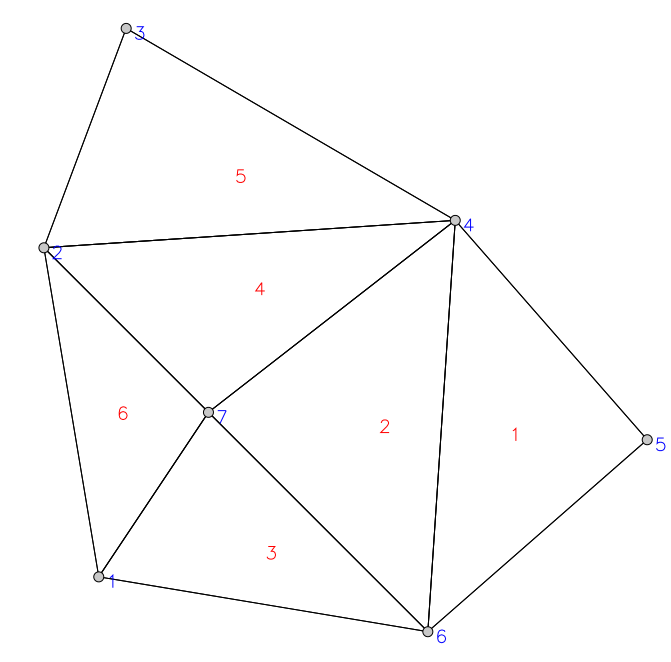
\includegraphics[width=0.9\textwidth]{../img/struct_triangulace.png}
\label{fig:struct_triangulace}
\end{figure}

\subsection{Jednoduchá trojúhelníková struktura}
Tato struktura ukládá informace v nejjednodušší podobě. Pracuje pouze s trojicemi id jednotlivých vrcholů trojúhelníků v seznamu nebo v poli. Trojúhelníky jsou seřazeny vzestupně podle id, zatímco na pořadí uložených vrcholů nezáleží. Struktura je velmi nenáročná, co se požadavků na kapacitu týče, nicméně toto je vykoupené tím, že nemáme k dispozici žádnou informaci, který trojúhelník sousedí s kterým.

\begin{table}[h]
\catcode`\-=12
\begin{tabular}{|c||c|c|c|}
\hline
\multirow{2}{*}{Trojúhelník} & \multicolumn{3}{c|}{Vrcholy} \\ \cline{2-4} 
                             & i        & j       & k       \\ \hline \hline
1                            & 4        & 6       & 5       \\ \hline
2                            & 7        & 6       & 4       \\ \hline
3                            & 1        & 6       & 7       \\ \hline
4                            & 2        & 7       & 4       \\ \hline
5                            & 2        & 4       & 3       \\ \hline
6                            & 2        & 1       & 7       \\ \hline
\end{tabular}
\end{table}



\subsection{Trojúhelníková struktura se sousedy}

Tato struktura přináší rozšíření o informaci, s kterými trojúhelníky daný trojúhelník sousedí. K zapotřebí je tedy další seznam, který obsahuje id trojúhelníku.

\begin{table}[h]
\catcode`\-=12
\begin{tabular}{|c||c|c|c||c|c|c|}
\hline
\multirow{2}{*}{Trojúhelník} & \multicolumn{3}{|c|}{Vrcholy} & \multicolumn{3}{|c|}{Sousedé}      \\ \cline{2-7} 
                             & i        & j       & k       & $t_{j,k}$ & $t_{k,i}$ & $t_{i,j}$ \\ \hline \hline
1                            & 4        & 6       & 5       & -         & -         & 2         \\ \hline
2                            & 7        & 6       & 4       & 1         & 4         & 3         \\ \hline
3                            & 1        & 6       & 7       & 2         & 6         & -         \\ \hline
4                            & 2        & 7       & 4       & 2         & 5         & 6         \\ \hline
5                            & 2        & 4       & 3       & -         & -         & 4         \\ \hline
6                            & 2        & 1       & 7       & 3         & 4         & -         \\ \hline
\end{tabular}
\end{table}


\subsection{Vertex-based struktura se sousedy}

Vertex-based struktura se sousedy je poměrně úsporná struktura, co se objemu dat týče. Ke každému vrcholu $v_i$ v síti jsou uloženy do seznamu sousedů vrcholy, které jsou s ním spojené. V případě že $v_i$ leží na konvexním obalu je seznam sousedů ukončen 'pseudovrcholem'. 

\begin{table}[h]
\catcode`\-=12
\begin{tabular}{|c||c|c|c|c|c|c||c|}
\hline
Vrchol & \multicolumn{6}{|c|}{Sousední vrcholy} & Suma vrcholů \\ \hline \hline
1      & 6    & 7    & 2    & 0    &     &     & 4            \\ \hline
2      & 1    & 7    & 4    & 3    & 0   &     & 9            \\ \hline
3      & 2    & 4    & 0    &      &     &     & 12           \\ \hline
4      & 3    & 2    & 7    & 6    & 5   & 0   & 18           \\ \hline
5      & 4    & 6    & 0    &      &     &     & 21           \\ \hline
6      & 5    & 4    & 7    & 1    & 0   &     & 26           \\ \hline
7      & 6    & 4    & 2    & 1    &     &     & 30           \\ \hline
\end{tabular}
\end{table}

\subsection{Half-edge datová struktura}
\subsection{Winged-edge datová struktura}
\subsection{Dart-based datová struktura}

\newpage
\section{Interpolace metodou přirozeného souseda}


\newpage
\section{Postup řešení}
\subsection{Bash}
Při řešení otázky, jak implementovat metodu přirozeného souseda pro GRASS 7, jsem vycházel z modulu napsaného pro GRASS GIS 6, který jsem měl k dispozici. Jednalo se o modul \textit{v.surf.nnbathy} pro vektorová data. Tento modul byl napsán v Bashi. Pro novou verzi GRASS GISu 7, ve které si vývojáři kladou za cíl zpřístupnit tento software širší veřejnosti, tento modul v Bashi ovšem nebylo možno použít, neboť do nové verze se počítá pouze s moduly v jazyce Python a C.

\subsubsection{v.surf.nnbathy}\footnote{\url{http://svn.osgeo.org/grass/grass-addons/grass6/raster/v.surf.nnbathy/description.html}}
\textit{v.surf.nnbathy} je modul napsaný v bashi. Slouží jako interface mezi \textit{nnbathy} z externí knihovny \textit{nn-c} a GRASS GISem. \textit{v.surf.nnbathy} nabízí celkem tři algoritmy interpolace. Defaultně je nastaven \textit{Watsonův algoritmus 	pro Sibsonovu interpolaci}. Další možností je \textit{Delaunayova triangulace} a poslední \textit{Bělikovův a Semenovův algoritmus pro nesibsonovu interpolaci}. Pro Delaunayvou triangulaci, která je základem pro všechny tři algoritmy, se využívá knihovny \textit{Triangle} napsanou Jonathanem Richardem Schewchukem. Parametry pro spuštění modulu jsou tyto (nepovinné v hranatých závorkách):
\begin{description}
\item[output] Proměnná typu \textit{string}, název výstupní rastrové mapy, jediný povinný parametr.
\item[input] Proměnná typu \textit{string}, název vstupní vektorové mapy.
\item[[file]] Proměnná typu \textit{string}, název vstupního souboru.
\item[[zcolumn]] Proměnná typu \textit{string}, název sloupce z atributové tabulky, jehož data budou použity pro interpolaci.
\item[[layer]] Proměnná typu \textit{integer}, nastavení, zda se jedná od 2D nebo 3D vektorová data.
\item[[where]] Proměnná typu \textit{string}, SQL where podmínka.
\item[[alg]] Proměnná typu \textit{string}, název použitého algoritmu.
\end{description}

Z výše uvedeného seznamu, lze vidět, že jako vstupní data je možné použít vektorovou mapu nebo textový soubor.

\todo[inline]{TODO Vlozit obrazek vstupni mapy a priklad vstupniho souboru}
\todo[inline]{Vkladat kod do vlastni prace??, nastaveni listing}

Volání v příkazové řádce pak může vypadata například takto:
\begin{lstlisting}[language=bash,caption={bash version}]
user@my_comp:~$ v.surf.nnbathy input=elevation_lid792_randpts@PERMANENT output=raster_map zcolumn=value alg=nn
\end{lstlisting}

%r.surf v bashi
\begin{comment}
\subsubsection{r.surf.nnbathy}\footnote{\url{http://svn.osgeo.org/grass/grass-addons/grass6/vector/r.surf.nnbathy/description.html}}
Modul \textit{r.surf.nnbathy} pracuje na podobném principu jako modul \textit{v.surf.nnbathy}, jen pro rastrová data. Při volání je možnost použít méně parametrů.
\begin{description}
\item[output] Proměnná typu \textit{string}, název výstupní rastrové mapy, jediný povinný parametr.
\item[input] Proměnná typu \textit{string}, název vstupní vektorové mapy.
\item[[alg]] Proměnná typu \textit{string}, název použitého algoritmu.
\end{description}

Volání v příkazové řádce pak může vypadata například takto:
\begin{lstlisting}[language=bash,caption={bash version}]
user@my_comp:~$ v.surf.nnbathy input=elevation_lid792_randpts@PERMANENT output=raster_map zcolumn=value alg=nn
\end{lstlisting}
\end{comment}

\newpage
\subsection{Python}
Jako první krok pro implementaci interpolace přirozeného souseda pro GRASS GIS 7 bylo potřeba stávající modul v bashi přepsat do podporovaného programovacího jazyka. Pro verzi 7 bylo možné napsat moduly buďto v jazyce C nebo Python. Z důvodu nepříliš velké zkušenosti v programování byl pro začátek zvolen jazyk Python, který je pro méně zkušené programátory vice přívětivý. 

\subsubsection{v.surf.nnbathy.py}
\todo[inline]{Z gitu stahnout kod bez objektu}
\begin{lstlisting}
\end{lstlisting}

V následující části této práce bude popsáno jak pythoní modul funguje, jaká jsou vstupní a výstupní data, jaké vytváří dočasné soubory.

\paragraph{Vstupní data}
Stejně jako původní bashový modul, i tento modul pracuje se vstupními daty buď v podobě textového ASCII souboru nebo vektorové mapy. Textový ASCII s \textit{n} body musí obsahovat \textit{n} řádků a 3 sloupce. V prvních dvou sloupcích je uložen údaj o poloze v podobě x a y souřadnice. Ve třetím sloupci jsou pak uloženy hodnoty veličiny, kterou chceme interpolovat.

%ukazka TMPXYZ
\begin{lstlisting}
638234.122902785427868 221198.4894384436775 62.817782000000001
638755.665974545176141 220976.783764891704777 9.190488000000000
638729.530741120455787 219988.669646041787928 91.799952000000005
638088.941303733270615 220228.186909802345326 76.839046999999994
638158.578729554312304 220794.514421981060877 2.037001000000000
637781.724264170858078 219988.193243810994318 8.298977000000001
638359.847223712014966 220692.375897407706361 15.550326000000000
639137.670258715632372 221096.622500944242347 16.613054999999999
637783.077698686625808 219603.568831721117022 38.046551000000001
639157.228799516917206 219692.376464909117203 82.820330999999996
\end{lstlisting}

Druhou možností vstupních dat je pak vektorová mapa s body. V tomto případě je pak při volání modulu použít parametr \textit{zcolumn}, který určuje z jakého sloupce atributové tabulky se budou brát hodnoty k interpolaci.


\paragraph{Funkce region()}
Každá operace prováděná v GRASS GISu je prováděna pouze na určitém rozsahu území, tzv. \textit{výpočetním regionu}. \textit{Výpočetní region} je určen jako obdélník daný mezními kartografickými souřadnicemi a počtem řádků a sloupců. 
Funkce \textit{region()} všechna nastavení uloží do proměných. Dále vypočte plochu výpočetního regionu. Na rozdíl od GRASS GISu, který jako mezní kartografické souřadnice bere vnější rohy rohových buněk obdélníku, knihovna \textit{nn-c} používá středy rohových buněk, a proto je třeba nastavení výpočetního regionu opravit o rozlišení buněk.


\paragraph{Funkce initials\_controls()}
Ve chvíli, kdy je nastavený výpočetní region,můžeme provést úvodní kontroly a přípravy před samotným výpočtem. Zejména zda plocha výpočetního regionu není nulová a je kde provádět interpolaci. Dále je třeba zajistit jednoznačné určení vstupních dat, tedy zda se bude pracovat s ASCII souborem nebo vektorovou mapou, a jejich kontrolu, popřípadě SQL podmínku. Také kontrolujeme zda z knihovny \textit{nn-c} máme nainstalovaný program \textit{nnbathy}, který interpolaci provádí. Také je třeba vytvořit dočasné pomocné soubory, které využijeme při práci s daty. 

V případě, že pracujeme s vektorovou mapu, uložíme informace o bodových datech do dočasného proměnné \textit{TMPcat} pomocí modulu \textit{v.out.ascii}. Výstupem toho modulu je ASCII soubor o \textit{n} řádcích a čtyřech sloupcích. V prvních dvou sloupcích je uložená poloha bodu, ve třetím jeho id a ve čtvrtém hodnota k interpolaci. 

%ukazka souboru TMPcat
\begin{lstlisting}
638234.122902785427868 221198.4894384436775 1 62.817782000000001
638755.665974545176141 220976.783764891704777 2 9.190488000000000
638729.530741120455787 219988.669646041787928 3 91.799952000000005
638088.941303733270615 220228.186909802345326 4 76.839046999999994
638158.578729554312304 220794.514421981060877 5 2.037001000000000
637781.724264170858078 219988.193243810994318 6 8.298977000000001
638359.847223712014966 220692.375897407706361 7 15.550326000000000
639137.670258715632372 221096.622500944242347 8 16.613054999999999
637783.077698686625808 219603.568831721117022 9 38.046551000000001
639157.228799516917206 219692.376464909117203 10 82.820330999999996
\end{lstlisting}

Jelikož id bodu k dalším výpočtům nepotřebujeme do dočasné proměnné \textit{TMPYZ} si uložíme pouze informace o poloze a hodnotu k interpolaci. V případě, že nepracujeme s vektorovou mapou, ale ASCII souborem, tak tento soubor rovnou uložíme do proměnné \textit{TMPXYZ}.



\paragraph{Funkce compute()}
V této části kódu je volán program \textit{nnbathy} s následujícími vstupními paramatry:
\begin{description}
\item[-w]{proměnná typu double, omezuje extrapolaci přiřezením minimální váhy pro vrchol Delaunayovi sítě. V našem případě nastavena nula, což zamezuje extrapolaci.}
\item[-i]{proměnná typu string, název vstupního souboru o \textit{n} řádcích, se třemi sloupci, x a y souřadnicí a hodnotou k interpolaci}
\item[-x]{dvojice $x_min$, $x^max$ typu double, mezní hodnoty výstupní mřížky}
\item[-y]{dvojice $x_min$, $x^max$ typu double, mezní hodnoty výstupní mřížky}
\item[-P]{proměnná typu string, použitá metoda interpolace}
\item[-n]{dvojice double x double, rozlišení výstupní mřížky}
\end{description}

%ukazka XYZout
\begin{lstlisting}
637725 221045 NaN
637735 221045 NaN
637745 221045 NaN
637755 221045 NaN
637765 221045 NaN
637775 221045 23.2274425578696
637785 221045 20.3234644594092
637795 221045 23.6841650075168
637805 221045 27.1014688330494
637815 221045 30.5774260647664
\end{lstlisting}

Výstupem z \textit{nnbathy} je soubor \textit{XYZout}. Obsahuje data o výstupní mřížce buňku po buňce ve třech sloupcích. V prvních dvou jsou x a y souřadnice, ve třetím vyinterpolovaná hodnota. V případě buňek mimo oblast, kde probíhala interpolace, je ve třetím sloupci uložena hodnota NaN.



\paragraph{Funkce convert()}
Výstupní textový soubor z \textit{nnbathy} je třeba upravit, aby s ním bylo možné dále pracovat v GRASS GISu. Pro další práci slouží dočasný soubor \textit{TMP}. Při vytváření na začátku tohoto souboru vznikne hlavička, která obsahuje data o hranicích, rozlišení, typu a hodnotě null.

%Ukázka hlavičky
\begin{lstlisting}
north: 228495.0
south: 215005.0
east: 644995.0
west: 630005.0
rows: 1350
cols: 1500
type: double
null: NaN
\end{lstlisting}

Dále je potřeba vybrat vyinterpolované hodnoty jednotlivých buněk ze souboru \textit{XYZout}, kde jsou uloženy ve třetím sloupci na samostatných řádcích, a vložit je do souboru \textit{TMP} v pravidelné mřížce.

%ukázka souboru TMP
\begin{lstlisting}
\end{lstlisting}

\paragraph{Funkce import\_to\_raster()}
Soubor \textit{TMP}, ve kterém máme uložené vyinterpolované hodnoty v pravidelné mřížce, slouží jako vstupní soubor pro modul \textit{r.in.ascii}, který tyto hodnoty převedu do rastru. Dále je použit modul \textit{r.support}, který uloží příkazy do rastrových metadat. Na závěr je vytištěna zpráva o, že byla vytvořena rastrová mapa.


\paragraph{Výstupní data}
Výstupem modulu \textit{v.surf.nnbathy} je rastrová mapa.
\todo[inline]{Vložit výstupní rastrovou mapu}

\newpage
\subsection{OOP}
V průběhu práce na přidání pythoního modulu \textit{v.surf.nnbathy} jsem zjistil, že v GRASS GISu verze 6 je k dispozici také bash modul \textit{r.surf.nnbathy}, který pracuje s rastrovými daty. Jelikož větší část kódu byla pro moduly v.surf.nnbathy a r.surf.nnbathy společná, rozhodl jsem se hlavní výpočetní část spojit. Na místo dvou procedurálních modulů byla objektově vytvořena knihovna \textit{nnbathy.py} a dva moduly \textit{v.surf.nnabthy.py} pro vektorová data a \textit{r.surf.nnbathy.py} pro data rastrová, které knihovnu \textit{nnbathy} volají.

\subsubsection{v.surf.nnbathy}
V objektově orientovaném modulu pro vektorová data, tak zůstaly úvodní část, která automaticky generuje GUI, úvodní vstupní kontroly a dále if podmínka, která vyhodnocovala, zda vstupují vektorová data v podobě vektorové mapy nebo ASCII souboru.



\subsubsection{r.surf.nnbathy}
Modul \textit{r.surf.nnbathy} pracuje na podobném principu jako modul \textit{v.surf.nnbathy}, jen pro rastrová data. Při volání je možnost použít méně parametrů.
\begin{description}
\item[output] Proměnná typu \textit{string}, název výstupní rastrové mapy, jediný povinný parametr.
\item[input] Proměnná typu \textit{string}, název vstupní vektorové mapy.
\item[[alg]] Proměnná typu \textit{string}, název použitého algoritmu.
\end{description}

Volání v příkazové řádce pak může vypadata například takto:
\begin{lstlisting}[language=bash,caption={bash version}]
user@my_comp:~$ v.surf.nnbathy input=elevation_lid792_randpts@PERMANENT output=raster_map zcolumn=value alg=nn
\end{lstlisting}

I v tomto modulu zůstala část, která vytváří GUI. Protože ale modul pracuje s daty pouze v podobě rastrové mapy nebyly potřeba žádně vstupní kontroly ani if podmínka.



\subsubsection{nnbathy}
V knihovně nnbathy, které oba moduly volají tedy zůstala hlavní výpočetní část kódu. 

\paragraph{Rodičovská třída Nnbathy} V rodičovské třídě NNbathy bylo vytvořeno několik objektů, které přebraly funkce jednotlivých procedur z předchozího kódu. Navíc byly vytvořeny tyto objekty:

\paragraph{Objekt \_\_init\_\_}
V tomto objektu se inicializují dočasné soubory a volá objekt region().


\paragraph{Objekt \_\_del\_\_}
Tento objekt slouží k odstranění dočasných souborů.

\paragraph{Třída Nnbathy\_raster}
Tato třída slouží pro rastrová vstupní data a je dědičná z rodičovské třídy Nnbathy.

\paragraph{Třída Nnbathy\_vector}
Tato třída slouží pro vektorová vstupní data a je dědičná z rodičovské třídy Nnbathy.

\paragraph{Třída Nnbathy\_file}
Tato třída slouží pro vstupní data v podobě ASCII souboru a je dědičná z rodičovské třídy Nnbathy.

\newpage
\section{Srovnání GRASSu a ostatních softwarů}




\begin{comment}
\newpage
\section{Interpolace přirozeným sousedem}

\todo[inline]{Prostudovat a probrat s T. Bayerem, po te opravit a doplnit!}

\subsection{Thiessenovy polygony}
\textit{Thiessenovy polygony} jsou sice samostatnou interpolační metodou, \textit{metoda přirozeného souseda} (MPS) je však využívá jako základ pro výpočet vah a proto bude jejich výpočet zmíněn i zde.

\textit{Thiessenovy polygony} známé taky jako \textit{Voronoiovy diagramy} jsou definovány takto: Nechť V je množina \textit{n} bodů v rovině. Rovinu rozdělíme na \textit{n} oblastí \textit{R} takových, že $R_i$ obsahuje všechny body z $E^2$, pro něž je bod $p_i  \in V$ nejbližší soused. Toto rozdělení roviny se nazývá Voronoiův diagram (VD) množiny bodů.

Nechť \textbf{A} = {$A_1,...,A_n$} je množina \textit{n} bodů. Voronoiův diagram $A_i$ je:\newline
$V(A_i)={X \in R^d : |X-A_i| \le |X-A_j| \forall _j = 1,...,n},$\newline kde $|X-A|$ vyjadřuje Eukleidovskou vzdálenost mezi body $X,A$ v prostoru $R^d$

VD má následující vlastnosti. Všechny oblasti jsou konvexní a oblast $R_i$ obsahuje jediný bod $p_i \in V$. Některé oblasti jsou neohraničené. Tyto obsahují body $p_i \in CH(V)$. Počet hran a uzlů VD je přímo úměrný počtu bodů v množině \textit{V}. Pokud žádné 4 body neleží na kružnici, uzly mají stupeň 3. Uzel VD leží ve středu kružnice určené 3 body z \textit{V}, které leží v přilehlých oblastech VD a neleží na přímce.
\bigskip
\textbf{Algoritmus konstrukce Voronoiova diagramu}

Množinu \textit{n} bodů v rovině rozdělíme svislou přímkou na dvě stejně velké podmnožiny \textit{V1} a \textit{V2}. Při dosažení malého počtu bodů zkonstruujeme VD1 a VD2 rozdělených množin , jinak dělení rekurzivně opakujeme. Po vyřešení dílčích VD spojujeme dvojice VD následujícím způsobem:

Nechť VD1 a VD2 kspi dva vypočítáné Voronoiovy diagramy množin oddělených hraniční svislou přímkou. Pro jejich spojení využijeme skutečnosti, že hrany výsledného VD patří buď zcela do VD1 nebo VD2, nebo leží na osách úseček, spojujících body z V1 a V2 (tzv. bisektory). Tyto hrany tvoří řetěz, který je monotónní ve směru osy \textit{y}.

Nalezneme konvexní obal sjednocených množin \textit{V1} a \textit{V2}. Nový konvexní obal obsahuje úsečky tečné k původním konvexním obalům. Sestrojíme bisektory těchto tečných úseček.

Nechť \textit{l} je bisektor horní úsečky, určené vrcholykonvexního obalu. Přímka \textit{l} leží současně v oblastech $R_i \subset VD1$ a $R_j \subset VD2$. Určíme místo, ve kterém \textit{l} opustí buď oblast $R_i$ nebo $R_j$  a vstoupí do oblasti $R_k$. Oblast $R_k$ patří buď k VD1, nebo k VD2 a obsahuje bod $p_k$. Na hranici ukončíme hranu \textit{l} a vytvoříme novou hranu, která leží na bisektoru bodů $p_k$ a zbývajícího bodu $p_i$ nebo $p_j$ (pokud opustíme oblast $R_j$ nebo $R_i$). 

Směrem dolů vytváříme další hrany VD a algoritmus ukončíme, pokud dosáhneme spodní polopřímkové hrany.

\textbf{Delaunayova triangulace}

Nechť \textit{V} je množina \textit{n} bodů. Předpokládáme, že žádné 4 body z \textit{V} neleží na kružnici. Pokud propojíme všechny sousední body určené Voronoiovým diagramem úsečkami, dostaneme triangulační síť, kterou studoval Delaunay v roce 1935. Tato triangulace je výhodná např. pro interpolaci, neboť minimalizuje délky hran trojúhelníků a zpřesňuje tak výpočty přírůstků. 

\subsection{Samotná interpolace}
MPS může být použita i pro bod \textit{x}, který není součástí množiny \textit{A}. V tomto případě přirození sousedé bodu \textit{A} jsou body z množiny \textit{A},jejichž Voronoiovy diagramy by byly pozměneny v případě, že by bod \textit{A} byl vložen do VD(\textit{S}).

Průnik \textit{x} vytvoří nový VD, který "ukrade" plochu VD, které by byly jeho přirozenými sousedy. 

\section{Skripty}
%r.surf.nnbathy v bashi kod
\begin{lstlisting}[language=bash,caption={bash version}]
#!/bin/sh

############################################################################
#
# MODULE:     v.surf.nnbathy
#
# AUTHOR(S):  Hamish Bowman, Otago University, New Zealand
#		Based on r.surf.nnbathy by Maciej Sieczka
#
# PURPOSE:    Interpolate raster surface using the "nnbathy" natural
#             neighbor interpolation program.
#
# COPYRIGHT:  (c) 2014 Hamish Bowman, Maciej Sieczka, and the GRASS Development Team
#
# LICENSE:    This program is free software under the GNU General Public
#             License (>=v2). Read the file COPYING that comes with GRASS
#             for details.
#
#############################################################################

# NOTES:
#
# 1. Requires nnbathy executable v 1.75 or later. Follow the instruction in
#    html manual page to obtain it.
#
# 2. When creating the input raster map, make sure it's extents cover
#    your whole region of interest, the cells you wish to interplate on are
#    NULL, and the resolution is correct. Same as most GRASS raster modules
#    this one is region sensitive too.


#%Module
#% description: Interpolates a raster map using the nnbathy natural neighbor interpolation program.
#%End
#%Option
#% key: input
#% type: string
#% gisprompt: old,vector,vector
#% description: Name of input vector points map
#% guisection: Selection
#% required : no
#%End
#%Option
#% key: output
#% gisprompt: new,cell,raster
#% type: string
#% description: Name for output raster map
#% required : yes
#%End
#%Option
#% key: zcolumn
#% type: string
#% required: no
#% multiple: no
#% description: Name of the attribute column with values to be used for approximation (if layer>0)
#% guisection: Selection
#%End
#%Option
#% key: layer
#% type: integer
#% required: no
#% multiple: no
#% label: Layer number
#% description: If set to 0, z coordinates are used. (3D vector only)
#% answer: 1
#% gisprompt: old_layer,layer,layer_zero
#% guisection: Selection
#%End
#%Option
#% key: where
#% type: string
#% required: no
#% multiple: no
#% key_desc: sql_query
#% label: WHERE conditions of SQL statement without 'where' keyword
#% description: Example: income < 1000 and inhab >= 10000
#% guisection: Selection
#%End
#%option
#% key: alg
#% type: string
#% options: l,nn,ns
#% answer: nn
#% descriptions: l;Linear;nn;Sibson natural neighbor;ns;Non-Sibsonian natural neighbor
#% description: Interpolation algorithm
#%End
#%Option
#% key: file
#% type: string
#% gisprompt: old_file,file,input
#% label: Name of input text file
#% description: Containing x,y,z data as three space separated columns
#% required : no
#%End


if [ -z "$GISBASE" ]; then
  echo "ERROR: You must be in GRASS GIS to run this program." 1>&2
  exit 1
fi

if [ "$1" != "@ARGS_PARSED@" ]; then
  exec g.parser "$0" "$@"
fi

if [ -n "$GIS_OPT_INPUT" ] && [ -n "$GIS_OPT_FILE" ] ; then
  g.message -e "Please specify either the 'input' or 'file' option, not both."
  exit 1
fi

if [ -z "$GIS_OPT_INPUT" ] && [ -z "$GIS_OPT_FILE" ] ; then
  g.message -e "Please specify either the 'input' or 'file' option."
  exit 1
fi

if [ -n "$GIS_OPT_FILE" ] && [ ! -e "$GIS_OPT_FILE" ] ; then
  g.message -e "File '$GIS_OPT_FILE' does not exist."
  exit 1
fi

# check if we have awk
if [ ! -x "`which awk`" ]; then
  g.message -e '"awk" executable required but not found.'
  exit 1
fi

# check if we have nnbathy
if [ ! -x "`which nnbathy`" ]; then
  g.message -e '"nnbathy" executable required but not found. Follow the instructions in v.surf.nnbathy manual to install.'
  exit 1
fi

# check nnbathy version
nnv=`nnbathy -v | sed 's/ /\n/g' | sort -nr | head -n1`
nnv_ok=`echo $nnv | awk '{ if ($0<1.76) {print 0} else {print 1} }'`

if [ $nnv_ok -eq 0 ]; then
  g.message -e '"nnbathy" version >= 1.76 is required.'
  exit 1
fi

# set up temporary files
TMP="`g.tempfile pid=$$`"
if [ $? -ne 0 ] || [ -z "$TMP" ]; then
  g.message -e 'Unable to create temporary files.' 1>&2
  exit 1
fi

# set environment so that awk works properly in all languages
unset LC_ALL
LC_NUMERIC=C
export LC_NUMERIC

PROG=`basename $0`

# define cleanup procedure
proc_cleanup() {
  # Reset traps before normal script termination to avoid bogus ERROR message, as
  # we put a trap on signal 0.
  trap - 0 2 3 15 
  rm -f "$TMP" "$TMP.$PROG.input_xyz" "$TMP.$PROG.output_xyz" "$TMP.$PROG.output_grd"
}

# define run-time error handling procedure
proc_runtime_error() {
  g.message -e "There was an error at the script's run time. Please try to debug the problem if you can and let the GRASS developers know."
  exit 1
}

# define user-break procedure
proc_user_break() {
  g.message -e "User break!"
  proc_cleanup
  exit 1
}

# set trap for when script terminates
trap "proc_runtime_error" 0

# trap user break
trap "proc_user_break" 2 3 15


# assign main variables from user's input
INPUT="$GIS_OPT_INPUT"
OUTPUT="$GIS_OPT_OUTPUT"
ALG="$GIS_OPT_ALG"


### DO IT ###

# Make script terminate (ie. emit signal 0) if any statement returns a
# non-0 value. Then we trap signal 0, which lets handle such errors.
# However, the trap on signal 0 must be reset before normal script
# termination to avoid a bogus ERROR message then - this is done in the
# cleanup procedure.
set -e

# grab the current region settings
eval `g.region -gu`

if [ -n "$GIS_OPT_INPUT" ] ; then
  # spit out coords + values to be interpolated
  ## FIXME: check if data is 3D or use output column
  # column=  (slow!!)
  TMPXYZ="$TMP.$PROG.input_xyz"
  
  if [ "$GIS_OPT_LAYER" -eq 0 ] ; then
    # 3D vector points
    LAYER=""
    COLUMN=""
  else
    LAYER="layer=$GIS_OPT_LAYER"
    if [ -n "$GIS_OPT_ZCOLUMN" ] ; then
      COLUMN="columns=$GIS_OPT_ZCOLUMN"
    else
      g.message -e "Name of z column required for 2D vector maps."
      exit 1
    fi
  fi

  if [ -n "$GIS_OPT_WHERE" ] ; then
    v.out.ascii -r input="$INPUT" output="$TMPXYZ" format=point fs=space \
       dp=15 where="$GIS_OPT_WHERE" $LAYER $COLUMN
  else
    v.out.ascii -r input="$INPUT" output="$TMPXYZ" format=point fs=space \
       dp=15 $LAYER $COLUMN
  fi

  if [ "$GIS_OPT_LAYER" -gt 0 ] ; then
    # crop away the cat column
    mv "$TMPXYZ" "$TMPXYZ.cat"
    cut -f1,2,4 -d' ' "$TMPXYZ.cat" > "$TMPXYZ"
    rm "$TMPXYZ.cat"
  fi

else
  TMPXYZ="$GIS_OPT_FILE"
fi


# set the working region for nnbathy (it's cell-center oriented)
nn_n=`echo $n | awk -v res="$nsres" '{printf "%.8f", $1 - res/2.0}'`
nn_s=`echo $s | awk -v res="$nsres" '{printf "%.8f", $1 + res/2.0}'`
nn_w=`echo $w | awk -v res="$ewres" '{printf "%.8f", $1 + res/2.0}'`
nn_e=`echo $e | awk -v res="$ewres" '{printf "%.8f", $1 - res/2.0}'`

null="NaN"
type="double"


#### interpolate
g.message '"nnbathy" is performing the interpolation now. This may take some time.'
g.message "Once it completes an 'All done.' message will be printed."


nnbathy -W 0 -P alg="$ALG" -n "${cols}x${rows}" \
	-x "$nn_w" "$nn_e" -y "$nn_n" "$nn_s" \
	-i "$TMPXYZ" \
       > "$TMP.$PROG.output_xyz"


# Y in "r.stats -1gn" output is in descending order, thus -y must be in
# MAX MIN order, not MIN MAX, for nnbathy not to produce a grid upside-down

# convert the X,Y,Z nnbathy output into a GRASS ASCII grid, then import with r.in.ascii:

# 1 create header
cat << EOF > "$TMP.$PROG.output_grd"
north: $n
south: $s
east: $e
west: $w
rows: $rows
cols: $cols
null: $null
type: $type
EOF

# 2 do the conversion
g.message "Converting nnbathy output to GRASS raster ..."

awk -v cols="$cols" '
BEGIN {col_cur=1; ORS=" "}
{
 if (col_cur==cols) {ORS="\n"; col_cur=0; print $3; ORS=" "}
		    else {print $3}
 col_cur++
}' "$TMP.$PROG.output_xyz" >> "$TMP.$PROG.output_grd"

# 3 import
r.in.ascii input="$TMP.$PROG.output_grd" output="$OUTPUT" --quiet

# store comand history in raster's metadata

if [ -n "$GIS_OPT_INPUT" ] ; then
  r.support map="$OUTPUT" history="v.surf.nnbathy alg=$ALG input=$INPUT output=$OUTPUT"
  #TODO: layer= where= zcolumn=
else
  r.support map="$OUTPUT" history="v.surf.nnbathy alg=$ALG input=$FILE output=$OUTPUT"
fi
r.support map="$OUTPUT" history=""
r.support map="$OUTPUT" history="nnbathy run syntax:"
r.support map="$OUTPUT" history=""
r.support map="$OUTPUT" history="nnbathy -W 0 -P alg=$ALG -n ${cols}x$rows "
r.support map="$OUTPUT" history="-x $nn_w $nn_e "
r.support map="$OUTPUT" history="-y $nn_n $nn_s "
r.support map="$OUTPUT" history="-i tmp_in > tmp_out"
r.support map="$OUTPUT" history=""

### ALL DONE ###

proc_cleanup

g.message "Done. <$GIS_OPT_OUTPUT> created."

\end{lstlisting}

\begin{lstlisting}[language=python, caption={python version}]
    def region():
        # set the region
        global area, ALG, nn_n, nn_s, nn_w, nn_e, null, ctype, cols, rows
        reg = grass.read_command("g.region", flags='p')
        kv = grass.parse_key_val(reg, sep=':')
        reg_N = float(kv['north'])
        reg_W = float(kv['west'])
        reg_S = float(kv['south'])
        reg_E = float(kv['east'])
        cols = int(kv['cols'])
        rows = int(kv['rows'])
        nsres = float(kv['nsres'])
        ewres = float(kv['ewres'])
        reg = (reg_N, reg_W, reg_S, reg_E)
        area = (reg_N-reg_S)*(reg_E-reg_W)
        ALG = options['algorithm']

        # set the working region for nnbathy (it's cell-center oriented)
        nn_n = reg_N - nsres/2
        nn_s = reg_S + nsres/2
        nn_w = reg_W + ewres/2
        nn_e = reg_E - ewres/2
        null = "NaN"
        ctype = "double"
\end{lstlisting}

%kod initial_controls()
\begin{lstlisting}[language=python, caption={python version}]
    def initial_controls():
        # setup temporary files
        global TMP, TMPcat, XYZout, TMPXYZ
        TMPXYZ = 'tmpxyz.txt'
        TMPcat = 'TMPcat.txt'
        TMP = grass.tempfile()
        #TMPcat = grass.tempfile()
        #TMPXYZ = grass.tempfile()
        XYZout = grass.tempfile()

        if (TMPcat or TMPXYZ or XYZout or TMP) is None:
            grass.fatal("Unable to create temporary files.")

        # other controls
        if not grass.find_program('nnbathy'):
            grass.fatal('nnbathy is not available')

        if (options['input'] and options['file']):
            grass.message("Please specify either the 'input' or 'file' option, not both.")

        if not(options['input'] or options['file']):
            grass.message("Please specify either the 'input' or 'file' option.")

        if (options['file'] and os.path.isfile(options['file'])):
            grass.message("File "+options['file']+" does not exist.")

        if area == 0:
            grass.fatal(_("xy-locations are not supported"))
            grass.fatal(_("Need projected data with grids in meters"))

        if not options['file']:
            if int(options['layer']) == 0:
                LAYER = ''
                COLUMN = ''
            else:
                LAYER = int(options['layer'])
                if options['zcolumn']:
                    COLUMN = options['zcolumn']
                else:
                    grass.message('Name of z column required for 2D vector maps.')

            if options['kwhere']:
                grass.run_command("v.out.ascii", flags='r', overwrite=1, input=options['input'], output=TMPcat, format="point", separator="space", precision=15, where=options['kwhere'], layer=LAYER, columns=COLUMN)
            else:
                grass.run_command("v.out.ascii", flags='r', overwrite=1, input=options['input'], output=TMPcat, format="point", separator="space", precision=15, layer=LAYER, columns=COLUMN)

            if int(options['layer']) > 0:
                fin = open(TMPcat, 'r')
                fout = open(TMPXYZ, 'w')
                try:
                    for line in fin:
                        parts = line.split(" ")
                        fout.write(parts[0]+' '+parts[1]+' '+parts[3])
                except:
                    grass.message("Invalid input!")
                fin.close()
                fout.close()
            else:
                grass.message("Z coordinates are used.")
        else:
            TMPXYZ = options['file']
\end{lstlisting}

%kod compute()
\begin{lstlisting}[language=python, caption={python version}]
def compute():
        grass.message('"nnbathy" is performing the interpolation now. This may take some time...')
        grass.verbose("Once it completes an 'All done.' message will be printed.")

        #nnbathy calling
        fsock = open(XYZout, 'w')
        #TODO zkontrolovat zarovnani
        grass.call(['nnbathy',
                         '-W', '%d' % 0,
                         '-i', '%s' % TMPXYZ,
                         '-x', '%d' % nn_w, '%d' % nn_e,
                         '-y', '%d' % nn_n, '%d' % nn_s,
                         '-P', '%s' % ALG,
                         '-n', '%dx%d' % (cols, rows)],
                         stdout=fsock)
        fsock.close()
\end{lstlisting}

\begin{lstlisting}[language=python, caption={python version}]
        grass.run_command('r.in.ascii', input=TMP, output=options['output'], quiet=True)

        # store comand history in raster's metadata
        if options['input']:
            grass.run_command('r.support', map=options['output'],
                              history="v.surf.nnbathy alg=%s input=%s output=%s" % (options['algorithm'], options['input'], options['output']))
        else:
            grass.run_command('r.support', map=options['output'],
                              history="v.surf.nnbathy alg=%s input=%s output=%s" % (options['algorithm'], options['file'], options['output']))

        grass.run_command('r.support', map=options['output'], history="\nnnbathy run syntax:\nnbathy -W %d -i %s -x '%d %d' -y '%d %d' -P %s -n %dx%d" % \
                              (0, TMPXYZ, nn_w, nn_e, nn_n, nn_s, ALG, cols,rows))
        grass.message("Done. Raster map <%s> created." % options['output'])
\end{lstlisting}

%ukazka v.surf.nnbathy
\begin{lstlisting}[language=python, caption={python version}]
import sys
import os

from grass.script.core import parser
import grass.script as grass

from nnbathy import Nnbathy_vector, Nnbathy_file


def main():
    # initial controls
    if (options['input'] and options['file']):
        grass.fatal("Please specify either the 'input' \
                    or 'file' option, not both.")

    if not(options['input'] or options['file']):
        grass.message("Please specify either the 'input' or 'file' option.")

    if (options['file'] and os.path.isfile(options['file'])):
        grass.message("File "+options['file']+" does not exist.")

    # vector or file input?
    if (options['input']):
        obj = Nnbathy_vector(options)
    else:
        obj = Nnbathy_file(options)

    obj.compute()
    obj.create_output()

if __name__ == "__main__":
    options, flags = parser()
    main()

\end{lstlisting}

%Kod r.surf.nnbathy
\begin{lstlisting}[language=python,caption={python version}]
import os
import sys

from grass.script.core import parser
import grass.script as grass

from nnbathy import Nnbathy_raster


def main():
    obj = Nnbathy_raster(options)
    obj.compute()
    obj.create_output()

if __name__ == "__main__":
    options, flags = parser()
    main()
\end{lstlisting}

%Ukazka __init__
\begin{lstlisting}[language=python,caption={python version}]

%Ukazka __del__
\begin{lstlisting}[language=python,caption={python version}]


    def __del__(self):
        # cleanup
        if self._tmp:
            os.remove(self._tmp)
        if self._tmpxyz:
            os.remove(self._tmpxyz)
        if self._xyzout:
            os.remove(self._xyzout)
        if self._tmpcat:
            os.remove(self._tmpcat)
\end{lstlisting}
def __init__(self, options):
        self._tmpxyz = grass.tempfile()
        self._xyzout = grass.tempfile()
        self._tmp = grass.tempfile()
        self._tmpcat = grass.tempfile()
        self.options = options
        self.region()
        pass
\end{lstlisting}

%Ukazka Nnbathy_raster
\begin{lstlisting}[language=python,caption={python version}]
class Nnbathy_raster(Nnbathy):
    # class for raster input
    def __init__(self, options):
        Nnbathy.__init__(self, options)
        self._load(options)

    def _load(self, options):
        # load input raster
        grass.run_command('r.stats', flags='1gn', input=options['input'],
                          output=self._tmpxyz, quiet=True, overwrite=True)
\end{lstlisting}

%Ukazka Nnbathy_vector
\begin{lstlisting}[language=python,caption={python version}]
class Nnbathy_vector(Nnbathy):
    # class for vector input
    def __init__(self, options):
        Nnbathy.__init__(self, options)
        self._load(options)

    def _load(self, options):
        # load input vector, initial controls
        if int(options['layer']) == 0:
            _layer = ''
            _column = ''
        else:
            _layer = int(options['layer'])
            if options['zcolumn']:
                _column = options['zcolumn']
            else:
                grass.message('Name of z column required for 2D vector maps.')

        # convert vector to ASCII
        if options['kwhere']:
            grass.run_command("v.out.ascii", flags='r', overwrite=1,
                              input=options['input'], output=self._tmpcat,
                              format="point", separator="space", dp=15,
                              where=options['kwhere'], layer=_layer,
                              columns=_column)
        else:
            grass.run_command("v.out.ascii", flags='r', overwrite=1,
                              input=options['input'], output=self._tmpcat,
                              format="point", separator="space", dp=15,
                              layer=_layer, columns=_column)

        # edit ASCII file, crop out one column
        if int(options['layer']) > 0:
            fin = open(self._tmpcat, 'r')
            fout = open(self._tmpxyz, 'w')
            try:
                for line in fin:
                    parts = line.split(" ")
                    fout.write(parts[0]+' '+parts[1]+' '+parts[3])
            except StandardError, e:
                grass.fatal_error("Invalid input: %s" % e)
            fin.close()
            fout.close()
        else:
            grass.message("Z coordinates are used.")
\end{lstlisting}

%Ukazka Nnbathy_file
\begin{lstlisting}[language=python, caption={python version}]
class Nnbathy_file:
    # class for file input
    def __init__(self, options):
        self.options = options
        self._load(options)

    def _load(self, options):
        # load input file
        self._tmpxyz = options['file']
\end{lstlisting}


\end{comment}

\end{document}
